\documentclass[12pt]{article}
\usepackage{setspace, graphicx, fullpage, amssymb, amsmath, epsfig, natbib, array, multirow, hyperref}
\usepackage{amsfonts, bm} 
\usepackage{dcolumn}
\usepackage{subfigure, float} 
\usepackage[margin=.5in]{geometry} 
\usepackage{verbatim}
\usepackage{url}
\usepackage{enumerate}
\newcolumntype{d}[1]{D{.}{.}{#1}} 

\begin{document}
	
	\begin{center}
		Update: 13 December 2016
	\end{center}

For this week, I got the Senate data compiled and used it to make figures and tables. I allow the figures to account for individual congresses and use the tables to show aggregate results for majority/minority and Democrat/Republican. These are Tables 1-6 and figures 1-3. I further added tables for the \verb|emIRT| only specification for the House. These are Tables 7 and 8. Additionally, I have restructured the House plots so that they will contain all coefficients and confidence intervals. The new plots for the House are Figures 4-6

What I found when going over the Senate data is that for Democrats, ideological extremism in the \verb|emIRT| model ranges from approximately $-6.5$ to approximately $6.5$. The other model specifications have this as an entirely negative value. It's likely that this has to do with the bit of code we added to ensure that the ideological scores for Democrats were less than those for Republicans. For this reason, in the tables and figures which have random reassignment of ``flip flop'' votes or the ``hybrid'' model specification, ideological extremism is higher for Democrats in increasingly negative values and in increasingly positive values for Republicans. I would need to do far more digging into the data to express with utmost confidence how we ought to interpret Democrat ideological extremism in the \verb|emIRT| only model.

\begin{table}
	\begin{center}
		\begin{tabular}{l c c }
			\hline
			& Democrat & Republican \\
			\hline
			ideological\_extremism        & $1.090^{***}$ & $4.682^{***}$ \\
			& $(0.277)$     & $(0.413)$     \\
			vote\_share:pres\_vote\_share & $-35.560$     & $60.472$      \\
			& $(23.978)$    & $(35.042)$    \\
			responsiveness\_noncalls      & $0.765^{***}$ & $0.869^{***}$ \\
			& $(0.041)$     & $(0.040)$     \\
			vote\_share                   & $5.991$       & $-20.610$     \\
			& $(12.028)$    & $(20.857)$    \\
			pres\_vote\_share             & $51.177^{**}$ & $-46.219^{*}$ \\
			& $(15.516)$    & $(21.565)$    \\
			chair                         & $0.847$       & $1.981^{*}$   \\
			& $(0.711)$     & $(0.815)$     \\
			south13                       & $-1.715^{**}$ & $1.441^{*}$   \\
			& $(0.623)$     & $(0.639)$     \\
			female                        & $1.978^{*}$   & $0.157$       \\
			& $(0.923)$     & $(1.219)$     \\
			afam                          & $3.366$       & $-11.453^{*}$ \\
			& $(3.373)$     & $(4.706)$     \\
			latino                        & $1.316$       & $2.806$       \\
			& $(3.326)$     & $(4.000)$     \\
			up\_for\_reelection           & $-0.743$      & $-1.509^{**}$ \\
			& $(0.511)$     & $(0.578)$     \\
			seniority                     & $-0.036$      & $0.245^{**}$  \\
			& $(0.073)$     & $(0.090)$     \\
			freshman                      & $-1.915^{**}$ & $2.875^{***}$ \\
			& $(0.714)$     & $(0.848)$     \\
			retiree                       & $-3.037$      & $0.656$       \\
			& $(3.783)$     & $(4.000)$     \\
			best\_committee               & $-0.059$      & $0.170$       \\
			& $(0.159)$     & $(0.182)$     \\
			leader                        & $2.932^{**}$  & $0.811$       \\
			& $(0.889)$     & $(0.861)$     \\
			power\_committee              & $-0.092$      & $1.396$       \\
			& $(0.969)$     & $(1.040)$     \\
			(Intercept)                   & $7.999$       & $-0.875$      \\
			& $(9.166)$     & $(13.353)$    \\
			\hline
			R$^2$                         & 0.541         & 0.535         \\
			Adj. R$^2$                    & 0.533         & 0.526         \\
			Num. obs.                     & 981           & 902           \\
			RMSE                          & 7.389         & 7.882         \\
			\hline
			\multicolumn{3}{l}{\scriptsize{$^{***}p<0.001$, $^{**}p<0.01$, $^*p<0.05$}}
		\end{tabular}
		\caption{Senate emIRT Party Calls}
	\end{center}
\end{table}

\begin{table}
	\begin{center}
		\begin{tabular}{l c c }
			\hline
			& Majority Party & Minority Party \\
			\hline
			ideological\_extremism        & $1.090^{***}$ & $4.682^{***}$ \\
			& $(0.277)$     & $(0.413)$     \\
			vote\_share:pres\_vote\_share & $-35.560$     & $60.472$      \\
			& $(23.978)$    & $(35.042)$    \\
			responsiveness\_noncalls      & $0.765^{***}$ & $0.869^{***}$ \\
			& $(0.041)$     & $(0.040)$     \\
			vote\_share                   & $5.991$       & $-20.610$     \\
			& $(12.028)$    & $(20.857)$    \\
			pres\_vote\_share             & $51.177^{**}$ & $-46.219^{*}$ \\
			& $(15.516)$    & $(21.565)$    \\
			chair                         & $0.847$       & $1.981^{*}$   \\
			& $(0.711)$     & $(0.815)$     \\
			south13                       & $-1.715^{**}$ & $1.441^{*}$   \\
			& $(0.623)$     & $(0.639)$     \\
			female                        & $1.978^{*}$   & $0.157$       \\
			& $(0.923)$     & $(1.219)$     \\
			afam                          & $3.366$       & $-11.453^{*}$ \\
			& $(3.373)$     & $(4.706)$     \\
			latino                        & $1.316$       & $2.806$       \\
			& $(3.326)$     & $(4.000)$     \\
			up\_for\_reelection           & $-0.743$      & $-1.509^{**}$ \\
			& $(0.511)$     & $(0.578)$     \\
			seniority                     & $-0.036$      & $0.245^{**}$  \\
			& $(0.073)$     & $(0.090)$     \\
			freshman                      & $-1.915^{**}$ & $2.875^{***}$ \\
			& $(0.714)$     & $(0.848)$     \\
			retiree                       & $-3.037$      & $0.656$       \\
			& $(3.783)$     & $(4.000)$     \\
			best\_committee               & $-0.059$      & $0.170$       \\
			& $(0.159)$     & $(0.182)$     \\
			leader                        & $2.932^{**}$  & $0.811$       \\
			& $(0.889)$     & $(0.861)$     \\
			power\_committee              & $-0.092$      & $1.396$       \\
			& $(0.969)$     & $(1.040)$     \\
			(Intercept)                   & $7.999$       & $-0.875$      \\
			& $(9.166)$     & $(13.353)$    \\
			\hline
			R$^2$                         & 0.541         & 0.535         \\
			Adj. R$^2$                    & 0.533         & 0.526         \\
			Num. obs.                     & 981           & 902           \\
			RMSE                          & 7.389         & 7.882         \\
			\hline
			\multicolumn{3}{l}{\scriptsize{$^{***}p<0.001$, $^{**}p<0.01$, $^*p<0.05$}}
		\end{tabular}
		\caption{Senate emIRT Party Calls}
	\end{center}
\end{table}

\begin{table}
	\begin{center}
		\begin{tabular}{l c c }
			\hline
			& Democrat & Republican \\
			\hline
			ideological\_extremism        & $-3.963^{***}$ & $1.047^{**}$   \\
			& $(0.742)$      & $(0.339)$      \\
			vote\_share:pres\_vote\_share & $-6.289$       & $-43.542$      \\
			& $(23.066)$     & $(32.976)$     \\
			responsiveness\_noncalls      & $0.833^{***}$  & $0.948^{***}$  \\
			& $(0.037)$      & $(0.028)$      \\
			vote\_share                   & $-0.814$       & $28.831$       \\
			& $(11.574)$     & $(19.634)$     \\
			pres\_vote\_share             & $34.210^{*}$   & $25.659$       \\
			& $(14.987)$     & $(20.200)$     \\
			chair                         & $-1.845^{**}$  & $-3.119^{***}$ \\
			& $(0.699)$      & $(0.767)$      \\
			south13                       & $-3.968^{***}$ & $-0.026$       \\
			& $(0.662)$      & $(0.606)$      \\
			female                        & $-0.389$       & $0.419$        \\
			& $(0.895)$      & $(1.138)$      \\
			afam                          & $4.232$        & $-8.500$       \\
			& $(3.273)$      & $(4.405)$      \\
			latino                        & $1.804$        & $-6.779$       \\
			& $(3.238)$      & $(3.770)$      \\
			up\_for\_reelection           & $-0.602$       & $-0.164$       \\
			& $(0.496)$      & $(0.547)$      \\
			seniority                     & $-0.015$       & $0.142$        \\
			& $(0.071)$      & $(0.085)$      \\
			freshman                      & $-0.679$       & $0.479$        \\
			& $(0.697)$      & $(0.807)$      \\
			retiree                       & $-2.201$       & $1.475$        \\
			& $(3.661)$      & $(3.772)$      \\
			best\_committee               & $-0.074$       & $0.273$        \\
			& $(0.154)$      & $(0.171)$      \\
			leader                        & $-1.444$       & $0.390$        \\
			& $(0.867)$      & $(0.814)$      \\
			power\_committee              & $0.388$        & $1.306$        \\
			& $(0.940)$      & $(0.980)$      \\
			(Intercept)                   & $-16.227$      & $-20.011$      \\
			& $(9.423)$      & $(12.232)$     \\
			\hline
			R$^2$                         & 0.632          & 0.657          \\
			Adj. R$^2$                    & 0.626          & 0.650          \\
			Num. obs.                     & 980            & 902            \\
			RMSE                          & 7.171          & 7.433          \\
			\hline
			\multicolumn{3}{l}{\scriptsize{$^{***}p<0.001$, $^{**}p<0.01$, $^*p<0.05$}}
		\end{tabular}
		\caption{Senate Party Calls, Randomly Reassign Flip Flop Votes}
	\end{center}
\end{table}


\begin{table}
	\begin{center}
		\begin{tabular}{l c c }
			\hline
			& Majority Party & Minority Party \\
			\hline
			ideological\_extremism        & $-3.963^{***}$ & $1.047^{**}$   \\
			& $(0.742)$      & $(0.339)$      \\
			vote\_share:pres\_vote\_share & $-6.289$       & $-43.542$      \\
			& $(23.066)$     & $(32.976)$     \\
			responsiveness\_noncalls      & $0.833^{***}$  & $0.948^{***}$  \\
			& $(0.037)$      & $(0.028)$      \\
			vote\_share                   & $-0.814$       & $28.831$       \\
			& $(11.574)$     & $(19.634)$     \\
			pres\_vote\_share             & $34.210^{*}$   & $25.659$       \\
			& $(14.987)$     & $(20.200)$     \\
			chair                         & $-1.845^{**}$  & $-3.119^{***}$ \\
			& $(0.699)$      & $(0.767)$      \\
			south13                       & $-3.968^{***}$ & $-0.026$       \\
			& $(0.662)$      & $(0.606)$      \\
			female                        & $-0.389$       & $0.419$        \\
			& $(0.895)$      & $(1.138)$      \\
			afam                          & $4.232$        & $-8.500$       \\
			& $(3.273)$      & $(4.405)$      \\
			latino                        & $1.804$        & $-6.779$       \\
			& $(3.238)$      & $(3.770)$      \\
			up\_for\_reelection           & $-0.602$       & $-0.164$       \\
			& $(0.496)$      & $(0.547)$      \\
			seniority                     & $-0.015$       & $0.142$        \\
			& $(0.071)$      & $(0.085)$      \\
			freshman                      & $-0.679$       & $0.479$        \\
			& $(0.697)$      & $(0.807)$      \\
			retiree                       & $-2.201$       & $1.475$        \\
			& $(3.661)$      & $(3.772)$      \\
			best\_committee               & $-0.074$       & $0.273$        \\
			& $(0.154)$      & $(0.171)$      \\
			leader                        & $-1.444$       & $0.390$        \\
			& $(0.867)$      & $(0.814)$      \\
			power\_committee              & $0.388$        & $1.306$        \\
			& $(0.940)$      & $(0.980)$      \\
			(Intercept)                   & $-16.227$      & $-20.011$      \\
			& $(9.423)$      & $(12.232)$     \\
			\hline
			R$^2$                         & 0.632          & 0.657          \\
			Adj. R$^2$                    & 0.626          & 0.650          \\
			Num. obs.                     & 980            & 902            \\
			RMSE                          & 7.171          & 7.433          \\
			\hline
			\multicolumn{3}{l}{\scriptsize{$^{***}p<0.001$, $^{**}p<0.01$, $^*p<0.05$}}
		\end{tabular}
		\caption{Senate Party Calls, Randomly Reassign Flip Flop Votes}
	\end{center}
\end{table}


\begin{table}
	\begin{center}
		\begin{tabular}{l c c }
			\hline
			& Democrat & Republican \\
			\hline
			ideological\_extremism        & $-3.954^{***}$ & $1.081^{**}$   \\
			& $(0.743)$      & $(0.349)$      \\
			vote\_share:pres\_vote\_share & $-7.781$       & $-39.437$      \\
			& $(23.158)$     & $(33.943)$     \\
			responsiveness\_noncalls      & $0.847^{***}$  & $0.949^{***}$  \\
			& $(0.037)$      & $(0.029)$      \\
			vote\_share                   & $0.341$        & $27.633$       \\
			& $(11.620)$     & $(20.209)$     \\
			pres\_vote\_share             & $35.232^{*}$   & $21.462$       \\
			& $(15.046)$     & $(20.791)$     \\
			chair                         & $-1.811^{*}$   & $-3.526^{***}$ \\
			& $(0.702)$      & $(0.789)$      \\
			south13                       & $-3.967^{***}$ & $0.090$        \\
			& $(0.664)$      & $(0.623)$      \\
			female                        & $-0.487$       & $0.973$        \\
			& $(0.899)$      & $(1.171)$      \\
			afam                          & $4.186$        & $-8.336$       \\
			& $(3.286)$      & $(4.534)$      \\
			latino                        & $1.450$        & $-6.362$       \\
			& $(3.250)$      & $(3.880)$      \\
			up\_for\_reelection           & $-0.585$       & $-0.164$       \\
			& $(0.498)$      & $(0.563)$      \\
			seniority                     & $-0.025$       & $0.194^{*}$    \\
			& $(0.071)$      & $(0.087)$      \\
			freshman                      & $-0.671$       & $0.824$        \\
			& $(0.700)$      & $(0.831)$      \\
			retiree                       & $-1.916$       & $1.002$        \\
			& $(3.676)$      & $(3.883)$      \\
			best\_committee               & $-0.080$       & $0.266$        \\
			& $(0.155)$      & $(0.176)$      \\
			leader                        & $-1.489$       & $0.322$        \\
			& $(0.870)$      & $(0.838)$      \\
			power\_committee              & $0.355$        & $1.463$        \\
			& $(0.943)$      & $(1.008)$      \\
			(Intercept)                   & $-18.053$      & $-19.064$      \\
			& $(9.457)$      & $(12.591)$     \\
			\hline
			R$^2$                         & 0.636          & 0.645          \\
			Adj. R$^2$                    & 0.629          & 0.638          \\
			Num. obs.                     & 980            & 902            \\
			RMSE                          & 7.200          & 7.651          \\
			\hline
			\multicolumn{3}{l}{\scriptsize{$^{***}p<0.001$, $^{**}p<0.01$, $^*p<0.05$}}
		\end{tabular}
		\caption{Senate Party Calls, Hybrid}
	\end{center}
\end{table}

\begin{table}
	\begin{center}
		\begin{tabular}{l c c }
			\hline
			& Majority Party & Minority Party \\
			\hline
			ideological\_extremism        & $-3.954^{***}$ & $1.081^{**}$   \\
			& $(0.743)$      & $(0.349)$      \\
			vote\_share:pres\_vote\_share & $-7.781$       & $-39.437$      \\
			& $(23.158)$     & $(33.943)$     \\
			responsiveness\_noncalls      & $0.847^{***}$  & $0.949^{***}$  \\
			& $(0.037)$      & $(0.029)$      \\
			vote\_share                   & $0.341$        & $27.633$       \\
			& $(11.620)$     & $(20.209)$     \\
			pres\_vote\_share             & $35.232^{*}$   & $21.462$       \\
			& $(15.046)$     & $(20.791)$     \\
			chair                         & $-1.811^{*}$   & $-3.526^{***}$ \\
			& $(0.702)$      & $(0.789)$      \\
			south13                       & $-3.967^{***}$ & $0.090$        \\
			& $(0.664)$      & $(0.623)$      \\
			female                        & $-0.487$       & $0.973$        \\
			& $(0.899)$      & $(1.171)$      \\
			afam                          & $4.186$        & $-8.336$       \\
			& $(3.286)$      & $(4.534)$      \\
			latino                        & $1.450$        & $-6.362$       \\
			& $(3.250)$      & $(3.880)$      \\
			up\_for\_reelection           & $-0.585$       & $-0.164$       \\
			& $(0.498)$      & $(0.563)$      \\
			seniority                     & $-0.025$       & $0.194^{*}$    \\
			& $(0.071)$      & $(0.087)$      \\
			freshman                      & $-0.671$       & $0.824$        \\
			& $(0.700)$      & $(0.831)$      \\
			retiree                       & $-1.916$       & $1.002$        \\
			& $(3.676)$      & $(3.883)$      \\
			best\_committee               & $-0.080$       & $0.266$        \\
			& $(0.155)$      & $(0.176)$      \\
			leader                        & $-1.489$       & $0.322$        \\
			& $(0.870)$      & $(0.838)$      \\
			power\_committee              & $0.355$        & $1.463$        \\
			& $(0.943)$      & $(1.008)$      \\
			(Intercept)                   & $-18.053$      & $-19.064$      \\
			& $(9.457)$      & $(12.591)$     \\
			\hline
			R$^2$                         & 0.636          & 0.645          \\
			Adj. R$^2$                    & 0.629          & 0.638          \\
			Num. obs.                     & 980            & 902            \\
			RMSE                          & 7.200          & 7.651          \\
			\hline
			\multicolumn{3}{l}{\scriptsize{$^{***}p<0.001$, $^{**}p<0.01$, $^*p<0.05$}}
		\end{tabular}
		\caption{Senate Party Calls, Hybrid}
	\end{center}
\end{table}



\begin{table}
	\begin{center}
		\begin{tabular}{l c c c c c c }
			\hline
			& Dem 97 & Dem 102 & Dem 107 & Rep 97 & Rep 102 & Rep 107 \\
			\hline
			(Intercept)                 & $-4.94$       & $46.05^{*}$   & $68.98^{***}$ & $-26.09^{***}$ & $-50.72^{***}$ & $52.85^{***}$ \\
			& $(5.46)$      & $(21.36)$     & $(6.70)$      & $(7.26)$       & $(11.86)$      & $(4.38)$      \\
			new\_ideological\_extremism & $1.50^{***}$  & $13.77^{***}$ & $7.68^{***}$  & $8.80^{***}$   & $6.48^{***}$   & $3.52^{***}$  \\
			& $(0.42)$      & $(2.28)$      & $(0.82)$      & $(0.63)$       & $(1.19)$       & $(0.51)$      \\
			new\_pfrate100              & $1.02^{***}$  & $1.01^{***}$  & $0.65^{***}$  & $0.60^{***}$   & $1.12^{***}$   & $0.32^{***}$  \\
			& $(0.05)$      & $(0.13)$      & $(0.06)$      & $(0.05)$       & $(0.09)$       & $(0.02)$      \\
			dpres\_pct                  & $0.11^{**}$   & $0.11^{*}$    & $-0.05$       & $-0.06$        & $-0.12$        & $-0.13^{***}$ \\
			& $(0.04)$      & $(0.05)$      & $(0.04)$      & $(0.05)$       & $(0.07)$       & $(0.02)$      \\
			south.x                     & $-4.15^{***}$ & $-4.86^{***}$ & $1.10$        & $-1.50$        & $2.54^{*}$     & $-0.95^{**}$  \\
			& $(0.84)$      & $(0.87)$      & $(0.96)$      & $(0.92)$       & $(1.04)$       & $(0.33)$      \\
			votepct.x                   & $-0.04$       & $-0.05$       & $0.01$        & $0.08^{*}$     & $0.00$         & $-0.04^{**}$  \\
			& $(0.03)$      & $(0.03)$      & $(0.04)$      & $(0.04)$       & $(0.03)$       & $(0.02)$      \\
			female.x                    & $-0.74$       & $0.37$        & $-0.76$       & $-2.40$        & $0.08$         & $-1.28^{**}$  \\
			& $(1.81)$      & $(1.36)$      & $(0.92)$      & $(1.56)$       & $(1.92)$       & $(0.48)$      \\
			afam.x                      & $1.85$        & $-2.29$       & $0.31$        &                & $0.34$         & $1.88$        \\
			& $(1.83)$      & $(1.75)$      & $(1.29)$      &                & $(5.17)$       & $(2.16)$      \\
			latino.x                    & $2.38$        & $2.51$        & $-0.11$       & $2.63$         & $-5.27$        & $1.61$        \\
			& $(2.56)$      & $(2.12)$      & $(1.39)$      & $(4.46)$       & $(5.38)$       & $(0.87)$      \\
			seniority.x                 & $-0.08$       & $0.11$        & $-0.24^{*}$   & $0.13$         & $0.18$         & $-0.04$       \\
			& $(0.11)$      & $(0.11)$      & $(0.10)$      & $(0.13)$       & $(0.14)$       & $(0.05)$      \\
			freshman.x                  & $-0.66$       & $0.63$        & $0.68$        & $4.01^{***}$   & $1.99$         & $-0.03$       \\
			& $(1.27)$      & $(1.33)$      & $(1.50)$      & $(1.04)$       & $(1.55)$       & $(0.47)$      \\
			retiree                     & $0.08$        & $0.62$        & $-0.23$       & $1.27$         & $-0.34$        & $-1.00$       \\
			& $(1.45)$      & $(1.03)$      & $(1.89)$      & $(1.46)$       & $(1.02)$       & $(0.64)$      \\
			bestgrosswart               & $0.09$        & $0.10$        & $0.16^{*}$    & $0.09$         & $-0.04$        & $0.08^{*}$    \\
			& $(0.08)$      & $(0.09)$      & $(0.08)$      & $(0.07)$       & $(0.11)$       & $(0.04)$      \\
			leader.x                    & $3.60$        & $-1.92$       & $1.72$        & $0.81$         & $-1.16$        & $0.24$        \\
			& $(2.54)$      & $(2.25)$      & $(1.81)$      & $(1.89)$       & $(1.93)$       & $(0.73)$      \\
			power.x                     & $1.75$        & $1.23$        & $-1.58$       & $-3.11^{**}$   & $0.05$         & $0.17$        \\
			& $(0.95)$      & $(1.03)$      & $(1.00)$      & $(1.05)$       & $(1.22)$       & $(0.37)$      \\
			chair.x                     & $2.38$        & $0.90$        & $4.53$        &                & $-0.11$        & $0.37$        \\
			& $(1.34)$      & $(1.52)$      & $(5.17)$      &                & $(5.09)$       & $(0.53)$      \\
			\hline
			R$^2$                       & 0.82          & 0.79          & 0.63          & 0.75           & 0.74           & 0.69          \\
			Adj. R$^2$                  & 0.81          & 0.78          & 0.60          & 0.73           & 0.71           & 0.67          \\
			Num. obs.                   & 229           & 261           & 207           & 185            & 159            & 211           \\
			RMSE                        & 4.78          & 5.50          & 4.75          & 4.36           & 4.94           & 1.89          \\
			\hline
			\multicolumn{7}{l}{\scriptsize{$^{***}p<0.001$, $^{**}p<0.01$, $^*p<0.05$}}
		\end{tabular}
		\caption{Who Heeds Table 3, emIRT House Party Calls}
	\end{center}
\end{table}

\begin{table}
	\begin{center}
		\begin{tabular}{l c c }
			\hline
			& Democrat & Republican \\
			\hline
			(Intercept)                 & $16.10^{***}$ & $-4.42^{*}$   \\
			& $(2.20)$      & $(2.19)$      \\
			new\_ideological\_extremism & $3.65^{***}$  & $5.58^{***}$  \\
			& $(0.21)$      & $(0.25)$      \\
			new\_pfrate100              & $0.90^{***}$  & $0.75^{***}$  \\
			& $(0.02)$      & $(0.02)$      \\
			dpres\_pct                  & $0.05^{***}$  & $-0.24^{***}$ \\
			& $(0.01)$      & $(0.02)$      \\
			south.x                     & $-4.02^{***}$ & $1.72^{***}$  \\
			& $(0.27)$      & $(0.30)$      \\
			votepct.x                   & $0.02^{*}$    & $-0.01$       \\
			& $(0.01)$      & $(0.01)$      \\
			female.x                    & $0.80^{*}$    & $-1.44^{**}$  \\
			& $(0.38)$      & $(0.52)$      \\
			afam.x                      & $0.32$        & $-2.06$       \\
			& $(0.45)$      & $(2.67)$      \\
			latino.x                    & $-0.62$       & $0.63$        \\
			& $(0.55)$      & $(1.07)$      \\
			seniority.x                 & $-0.10^{**}$  & $-0.09$       \\
			& $(0.03)$      & $(0.05)$      \\
			freshman.x                  & $0.13$        & $0.72$        \\
			& $(0.36)$      & $(0.41)$      \\
			retiree                     & $-0.87$       & $-0.44$       \\
			& $(0.49)$      & $(0.54)$      \\
			bestgrosswart               & $0.07^{*}$    & $0.12^{***}$  \\
			& $(0.03)$      & $(0.03)$      \\
			leader.x                    & $0.95$        & $1.20$        \\
			& $(0.66)$      & $(0.67)$      \\
			power.x                     & $1.13^{***}$  & $-0.35$       \\
			& $(0.31)$      & $(0.37)$      \\
			chair.x                     & $2.69^{***}$  & $2.76^{***}$  \\
			& $(0.50)$      & $(0.71)$      \\
			\hline
			R$^2$                       & 0.69          & 0.58          \\
			Adj. R$^2$                  & 0.69          & 0.58          \\
			Num. obs.                   & 3982          & 3140          \\
			RMSE                        & 6.71          & 7.01          \\
			\hline
			\multicolumn{3}{l}{\scriptsize{$^{***}p<0.001$, $^{**}p<0.01$, $^*p<0.05$}}
		\end{tabular}
		\caption{Aggregate Results, emIRT House Party Calls}
	\end{center}
\end{table}
	
\begin{figure}[h]
	\caption{Figure 2 - Senate emIRT Only}
	\centering
	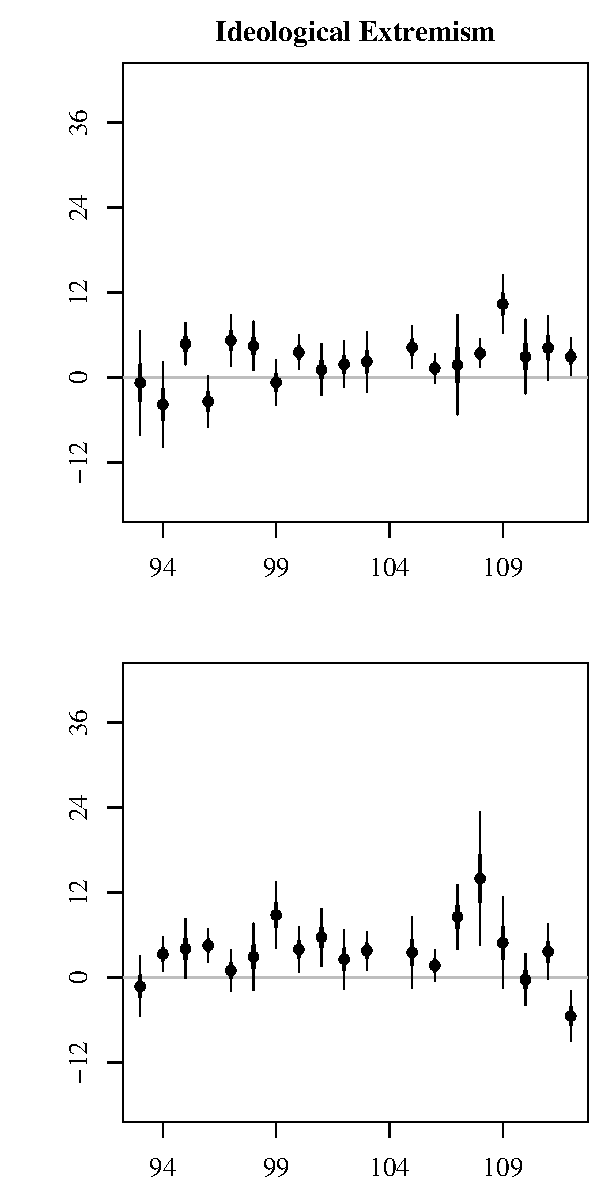
\includegraphics[]{C:/Users/Ethan/Documents/GitHub/partycalls/plots/who-heeds-figure2-senate_emIRT_only.pdf}
	
\end{figure}	

\begin{figure}[h]
	\caption{Figure 2 - Senate Randomly Reassign Flip Flop Votes}
	\centering
	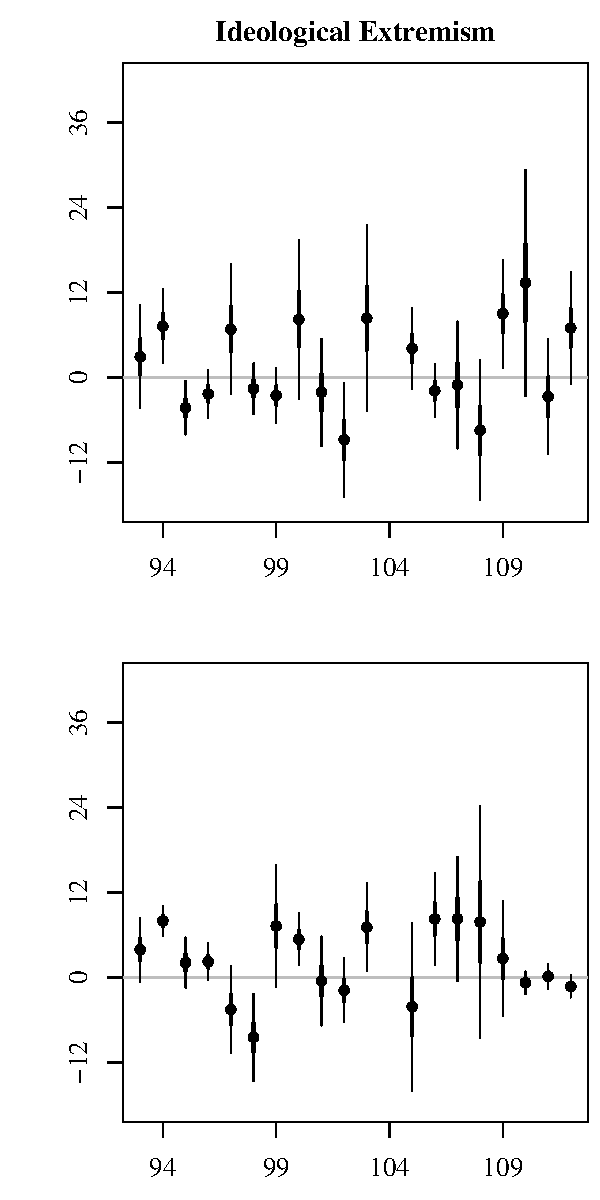
\includegraphics[]{C:/Users/Ethan/Documents/GitHub/partycalls/plots/who-heeds-figure2-senate_randomly_reassign_flip_flop_votes.pdf}
	
\end{figure}	
	
\begin{figure}[h]
	\caption{Figure 2 - Senate Hybrid}
	\centering
	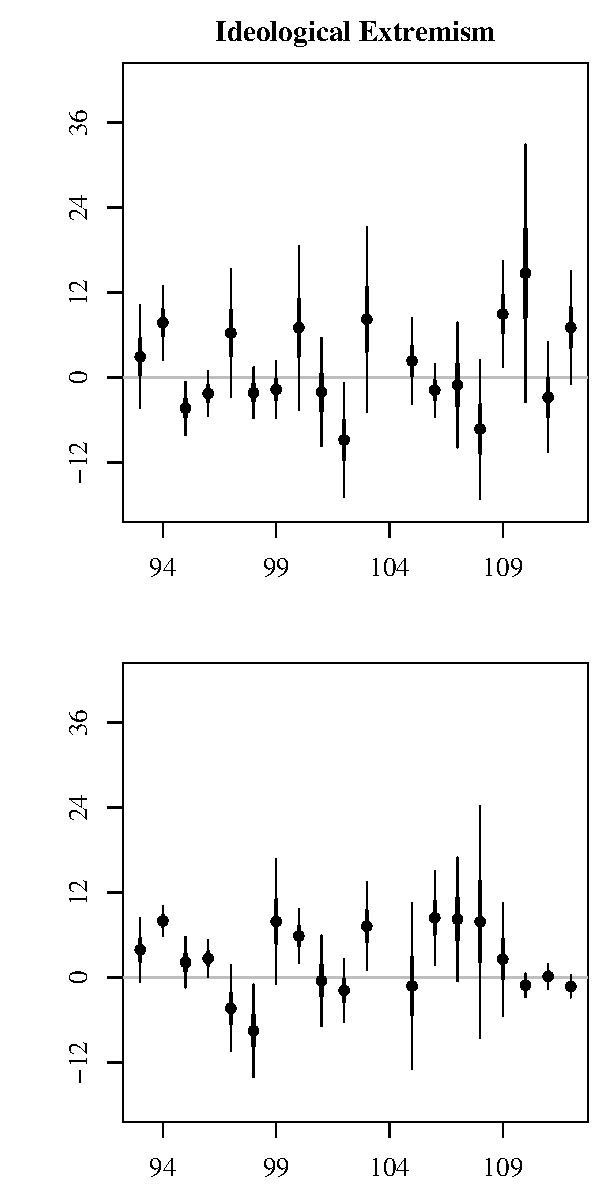
\includegraphics[]{C:/Users/Ethan/Documents/GitHub/partycalls/plots/who-heeds-figure2-senate_hybrid.pdf}
	
\end{figure}
	
\begin{figure}[h]
	\caption{Figure 2 - House emIRT Only}
	\centering
	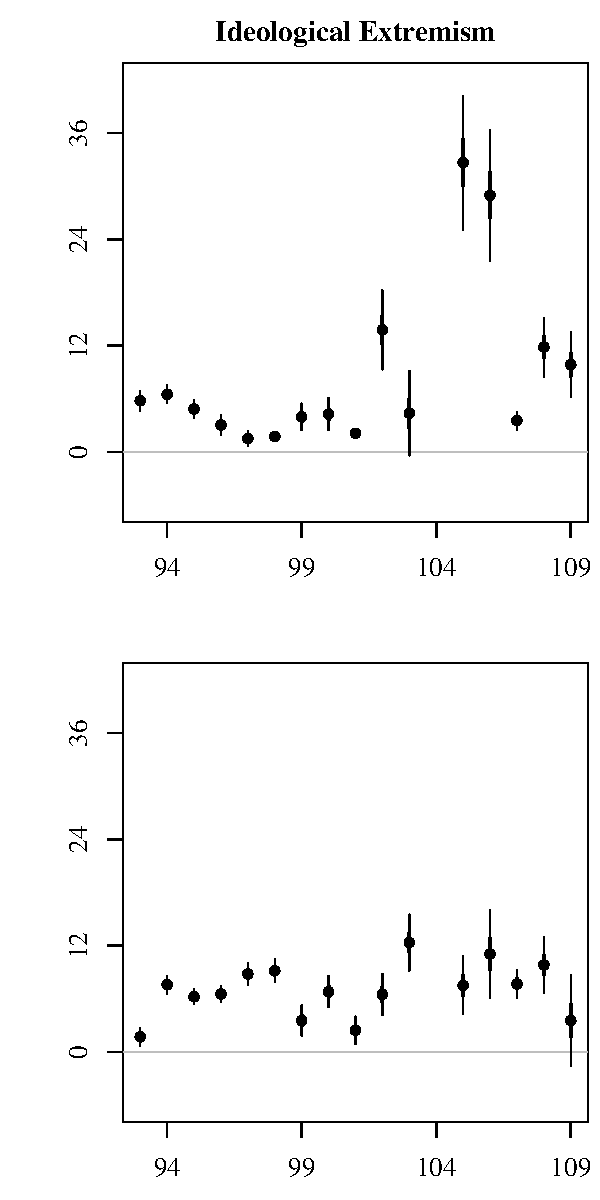
\includegraphics[]{C:/Users/Ethan/Documents/GitHub/partycalls/plots/who-heeds-figure2-replication_emIRT_only.pdf}
	
\end{figure}
	
\begin{figure}[h]
	\caption{Figure 2 - House Randomly Reassign Flip Flop Votes}
	\centering
	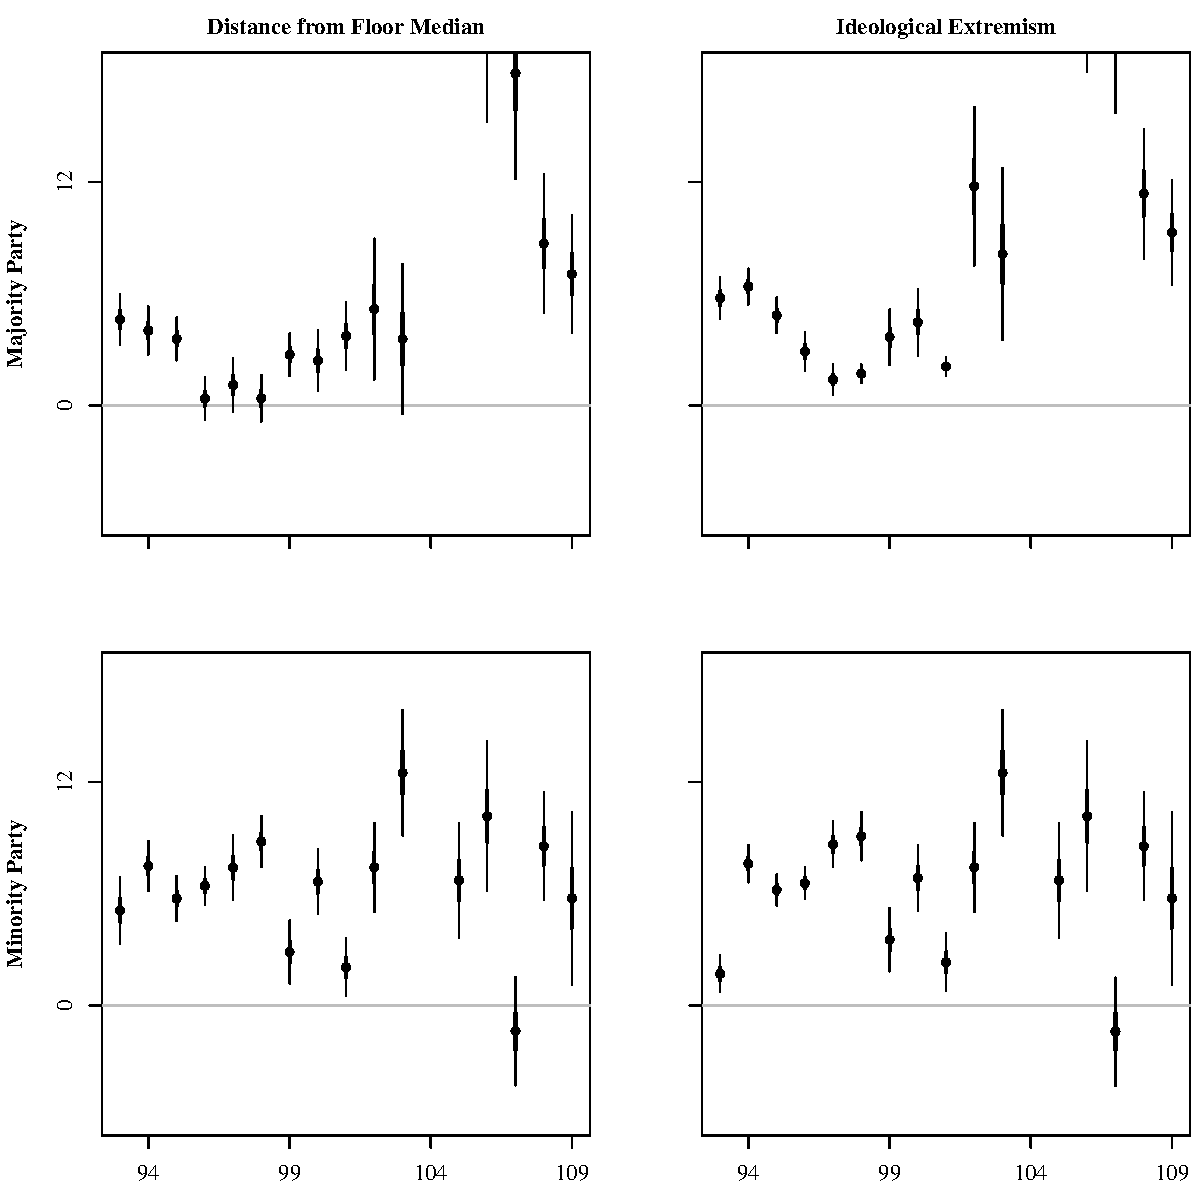
\includegraphics[]{C:/Users/Ethan/Documents/GitHub/partycalls/plots/who-heeds-figure2-replication_reassign_flip_flop_votes.pdf}
	
\end{figure}

\begin{figure}[h]
	\caption{Figure 2 - House Hybrid}
	\centering
	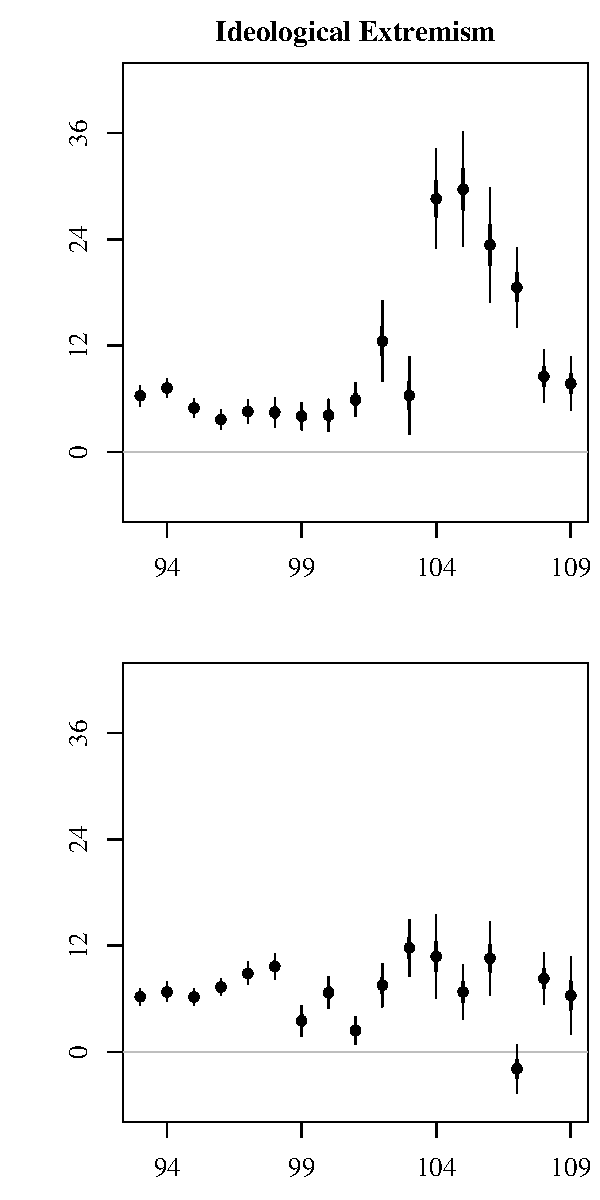
\includegraphics[]{C:/Users/Ethan/Documents/GitHub/partycalls/plots/who-heeds-figure2-replication_hybrid.pdf}
	
\end{figure}	

\end{document}